\section{Image-based control systems}
Cameras are now an integral part of modern (industrial) systems and are becoming increasingly popular in mixed-criticality systems.
A mixed-criticality system is a system that can execute several applications of different criticality levels - safety-critical, mission-critical and low-critical \cite{burns2013mixed}.
The criticality levels are formally defined, for example, as safety integrity levels in the IEC 61508 standard \cite{bell2006introduction} and \glspl{asil} in the automotive ISO 26262 standard \cite{jeon2011automotive}.
The versatility of the camera sensor allows an image captured by a single camera sensor to be used for multiple mixed-criticality applications.
In the automotive domain, for example, cameras are used to perceive the surrounding environment, enabling safety-critical autonomous driving and use for non-critical applications like drive recording.

\Gls{ibc} systems are a class of data-intensive feedback control systems whose feedback is provided by image-based sensing using cameras as sensors. 
Data-intensive feedback control systems are common nowadays due to advancements in \glspl{cps} \cite{van2018data}.
\Gls{ibc} systems have become popular with the advent of efficient image processing algorithms and low-cost \gls{cmos} cameras with high resolution \cite{corke2017robotics}. 
The combination of the camera and the image-processing algorithm gives necessary information on parameters such as relative position, geometry, relative distance, depth perception and tracking of the object-of-interest. 
This enables the effective use of low-cost camera sensors to enable new functionality or replace expensive sensors in cost-sensitive industries like automotive \cite{corke2017robotics,pendleton2017perception,saidi2018future}.
Applications of \gls{ibc} are found in robotics \cite{corke2017robotics}, autonomous vehicles \cite{elfring2016effective,pendleton2017perception}, advanced driver assistance systems (ADAS) \cite{bengler2014three}, electron microscopes \cite{FEI}, visual navigation \cite{chakraborty2016compensating} and so on.

The popularity of modern \gls{ibc} systems can be attributed to 
\begin{itemize}
    \item the impact of Moore's law \cite{moore1998cramming} and the constant breakthroughs in semiconductor manufacturing technology. This enabled the availability of powerful multiprocessors at relatively low cost and size, and also paved the way for the miniaturisation of \gls{cmos} cameras.
    \item the availability of low-cost high-resolution \gls{cmos} cameras with good quality and small size.
    \item the versatility of the camera images and the breakthroughs in \gls{ai} technology and deep-learning algorithms \cite{lecun2015deep}. Using deep-learning methods and algorithms, a multitude of features can be efficiently extracted from camera images and used for a variety of mixed-criticality applications.  
    \item the industrial adoption of heterogeneous platforms and the breakthroughs in \glspl{gpu} and \glspl{npu}. Examples of such developments are Tesla's \gls{fsd} computer \cite{talpes2020compute} and NVIDIA's Drive AGX platform \cite{nvidiadrive}. 
   The  \gls{fsd} computer is based on a \gls{soc} that integrates industry standard components such as \glspl{cpu}, \gls{isp}, \glspl{gpu}, and \glspl{npu}.
\end{itemize}

\begin{figure}[htb]
\centerline{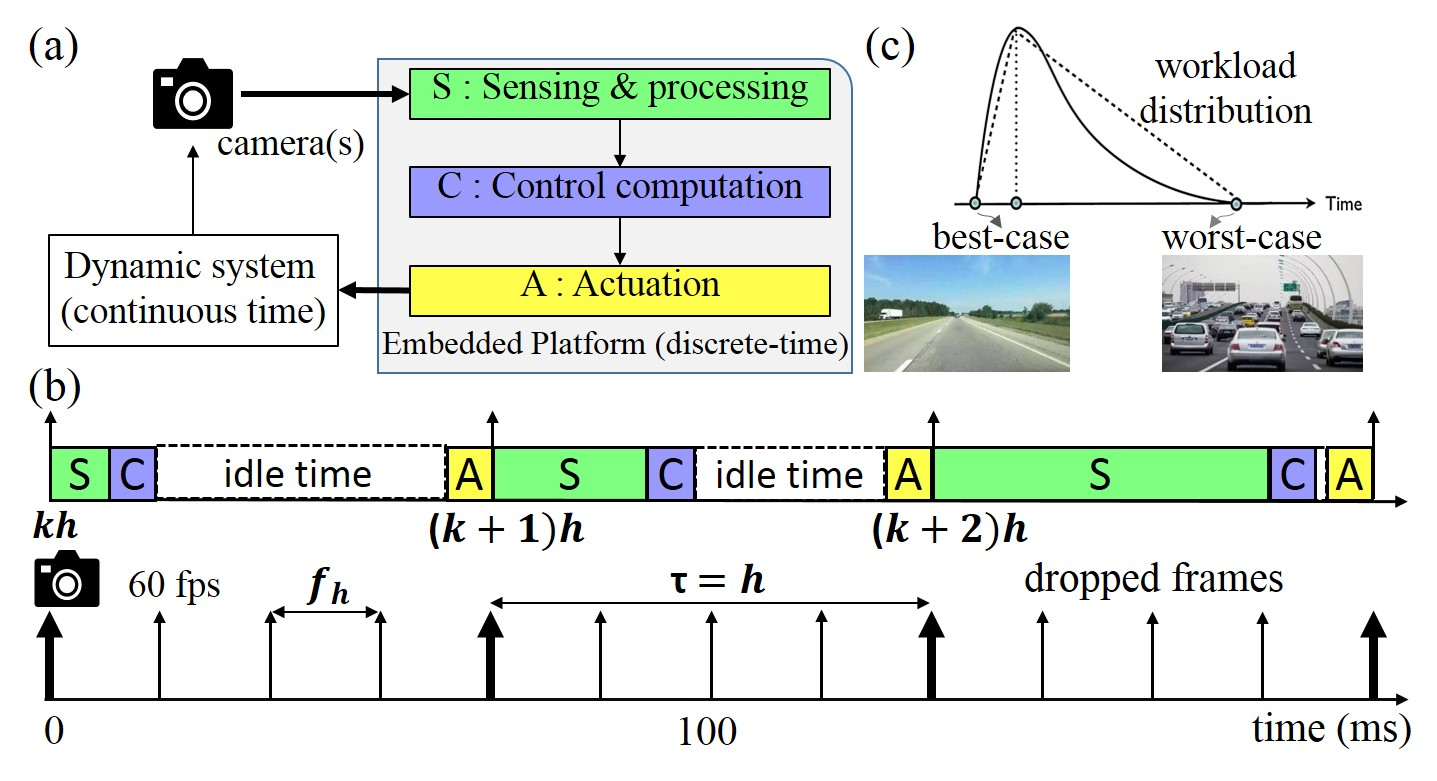
\includegraphics[width=\textwidth]{01_intro/images/ibc_intro.jpg}}
\vspace{-1ex}
\caption{An \acrfull{ibc} system: (a) block diagram; (b) Gantt chart for a typical \gls{ibc} implementation; (c) workload variations captured as a distribution. In the context of the thesis, workload refers to the image workload (unless specified differently). Image workload refers to the number of features in the image that should be processed. For example, more features in an image typically implies a higher workload.}
\label{fig:ch1_ibc_intro}
%\vspace{-2em}
\end{figure}

In this thesis, the focus is on \gls{ibc} systems that are functionally critical and on feedback control systems whose state is measured by the image-based sensing and processing, i.e., state feedback.
The case study of an automotive \gls{lkas} system is used to explain the concepts and results of this thesis.
A typical \gls{ibc} system is illustrated in Fig. \ref{fig:ch1_ibc_intro} (a).
A camera captures image frames at a pre-defined constant frames per second $\fps$, i.e., the frame rate, from the dynamic system environment (with the camera frame-arrival period $\fh$ $=\frac{1}{\fps}$).
An \gls{isp} processes the RAW camera image frames in the Bayer domain and converts it to the standard RGB image format, e.g. JPEG. 
Then, a compute-intensive image-processing algorithm processes the image frames to detect features in the image such as objects, traffic signs and lanes.
These features are then used to compute the states of the system, such as relative position and distance \cite{corke2017robotics}.
A controller computes the control input for actuation (e.g., change in direction) using the computed states.
The actuation task applies the computed control input to the \gls{ibc} system.

A typical feedback control implementation sequentially and
periodically (with sampling period $h$) executes the sensing and processing task (S), control compute task (C) and the actuating task (A) (as illustrated in Fig. \ref{fig:ch1_ibc_intro} (b)).
In an \gls{ibc} system, the sensing task may have a long, variable execution time and incur a long sensing delay. 
Variability in execution time may occur due to variation in image-processing workload and/or in the platform load caused by other applications.
The key \textit{challenge} is to deal with this \textit{high dynamic computation demand while guaranteeing performance and meeting safety requirements} such as stability.
A long variable processing delay results in dropping some camera frames from processing. 

These variations can be captured statistically using a probability distribution \cite{adyanthaya2014robustness} (illustrated in Fig. \ref{fig:ch1_ibc_intro} (c)).
It is interesting to note that this delay distribution is platform-dependent.
Platform-related parameters - for instance, number of processing cores, processor clock speed, memory, and communication bandwidth - have a direct impact on the observed delay. 
A long worst-case sensing delay leads to a long sensor-to-actuator delay $\tau$ (the time between the start of a sensing task and the end of the corresponding actuation task) and thus results in degraded control performance \cite{sharkey1996delays,aastrom2013computer}.

In this thesis, we develop approaches to cope with a long variable sensing delay exploiting the benefits of a multiprocessor platform and the application-specific \gls{ibc} system characteristics.
The platform-aware aspects explored in this thesis that exploit the benefits of a multiprocessor platform are - application parallelisation and pipelining of the control loop.
Parallelisation refers to executing sensing subtasks in parallel and thereby reducing the delay compared to the sequential implementation. 
Pipelining refers to the pipelined execution of the control loop over multiple processing cores thereby reducing the effective sampling period (the time between the start of two successive sensing tasks).
The two application-specific characteristics we exploit are - the image workload variations and approximate computing. 
Image workload variations occur due to the variations in the number of features in the captured images and the platform load. 
Approximate computing trades off accuracy in the signal processing for gains in response time and energy.